\documentclass[handout]{beamer}
\usetheme{Dresden}
\usecolortheme{beaver}

\usepackage[polish]{babel}
\usepackage[utf8]{inputenc}
\usepackage[T1]{fontenc}

\usepackage{subcaption}

\title{AntiSocialNetwork}
\subtitle{Projekt z baz danych}
\author[D. Benecki]{Damian Benecki}
\institute{Uniwersytet Wrocławski}
\date{\today}

\begin{document}
        \maketitle
        \begin{frame}
            \tableofcontents
        \end{frame}
    \section{Wprowadzenie}
        \begin{frame}
            \begin{itemize}
                \item Celem projektu było stworzenie nieskomplikowanej sieci społecznościowej \pause
                \item Pomysł został zainspirowany wykładem KNMT na temat grafów losowych \pause
                \item Był też pretekstem do stworzenia mechanizmu logowania, nauczenia się technologii webowych \pause
                \item Początkowo robiłem go z Janem Hickiewiczem, ale drogi nasze się rozeszły \pause
                \item Projekt udało się doprowadzić do końca i został nazwany \textit{AntiSocialNetwork}
            \end{itemize}
        \end{frame}
        \begin{frame}{Funkcjonalność}
            \begin{itemize}
                \item Możliwość tworzenia postów i komentarzy, zawierania znajomości oraz wysyłania wiadomości między sobą \pause
                \item Funkcjonalna strona rejestracji i logowania \pause
                \item Wyszukiwanie postów i użytkowników na podstawie wspólnych tematów \pause
                \item Hasła przechowywane w tabeli są zaszyfrowane
            \end{itemize}
        \end{frame}
        \section{Tabele}
        \begin{frame}[fragile]{Lista tabel}
            \begin{enumerate}
                \item \verb|login_credentials| -- odpowiada za logowanie się do serwisu \pause
                \item \verb|users| -- dane użytkownika np. nazwa, data urodzenia, płeć \pause
                \item \verb|countries| -- typ enumeracyjny, lista państw \pause
                \item \verb|posts| -- posty tworzone przez użytkowników \pause
                \item \verb|comments| -- komentarze do postów \pause
                \item \verb|likes| -- polubienia postów, pokazujące ich popularność \pause
                \item \verb|friend_requests| -- zapytania o znajomość \pause
                \item \verb|friends_with| -- zaakceptowane znajomości \pause
                \item \verb|messages| -- prywatne wiadomości pomiędzy znajomymi \pause
                \item \verb|tag_list| -- typ enumeracyjny, tagi ułatwiające wyszukiwanie \pause
                \item \verb|post_tags| -- przypisania tagów do postów \pause
                \item \verb|interests| -- tagi, którymi interesuje się użytkownik
            \end{enumerate}
        \end{frame}
        \begin{frame}[fragile]{Diagram tabel}
            \begin{figure}
                \centering   %timestamp zamiast date, country_name długości 51 
                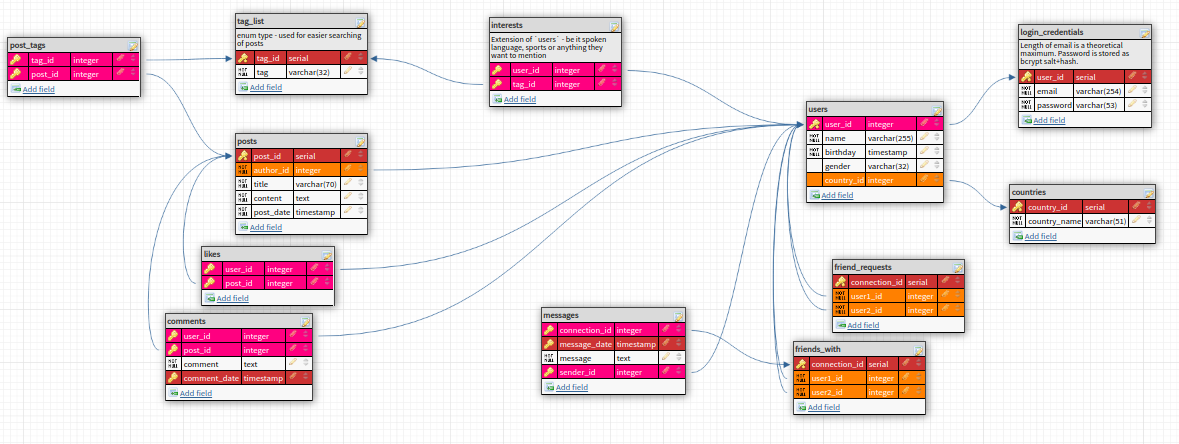
\includegraphics[width=\textwidth]{database_diagram.png}
            \end{figure}
        \end{frame}
        \begin{frame}[fragile]{Lista widoków}
            \begin{enumerate}
                \item \verb|n_comments_per_post| -- Ile każdy post ma komentarzy \pause
                \item \verb|n_likes_per_post| -- Ile każdy post ma polubień \pause
                \item \verb|n_friends_per_user| -- Ile każdy użytkownik ma znajomych \pause
                \item \verb|show_posts| -- Dane postów wyświetlane w liście postów \pause
            \end{enumerate}
            
            (Nie ma więcej widoków typu \verb|show_posts|, bo niezręcznie obsługuje się je programistycznie)
        \end{frame}
    \section{Przewodnik}
        
        \begin{frame}[fragile]{Strona startowa -- Rejestracja}
            \begin{figure}
                \centering
                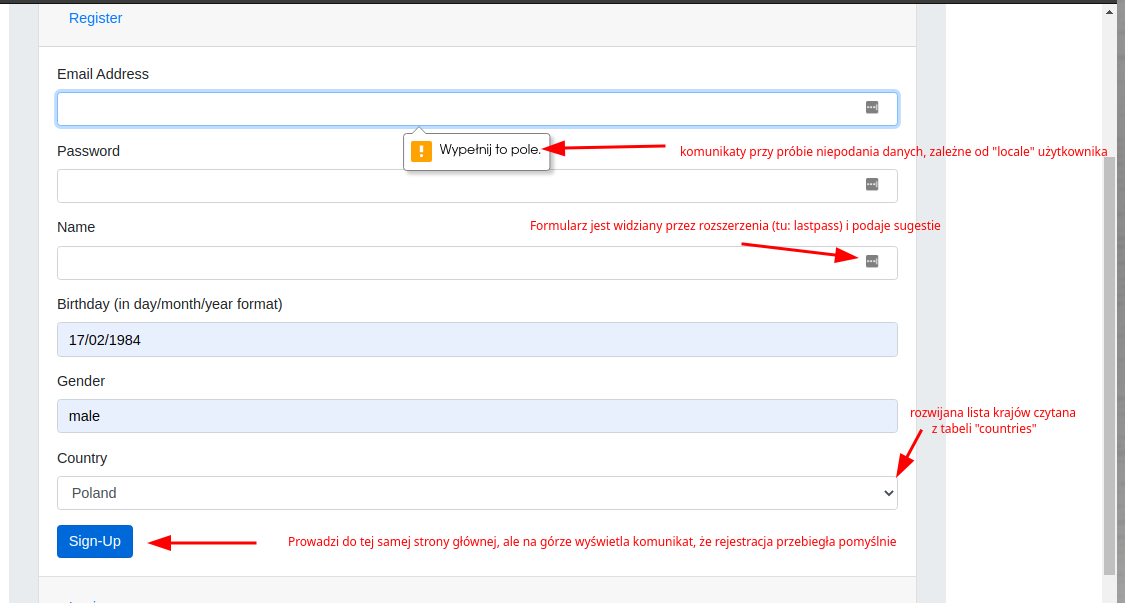
\includegraphics[width=\linewidth]{welcome_page_register.png}
            \end{figure}
        \end{frame}
        
        \begin{frame}[fragile]{Strona startowa -- Logowanie}
            \begin{figure}
                \centering
                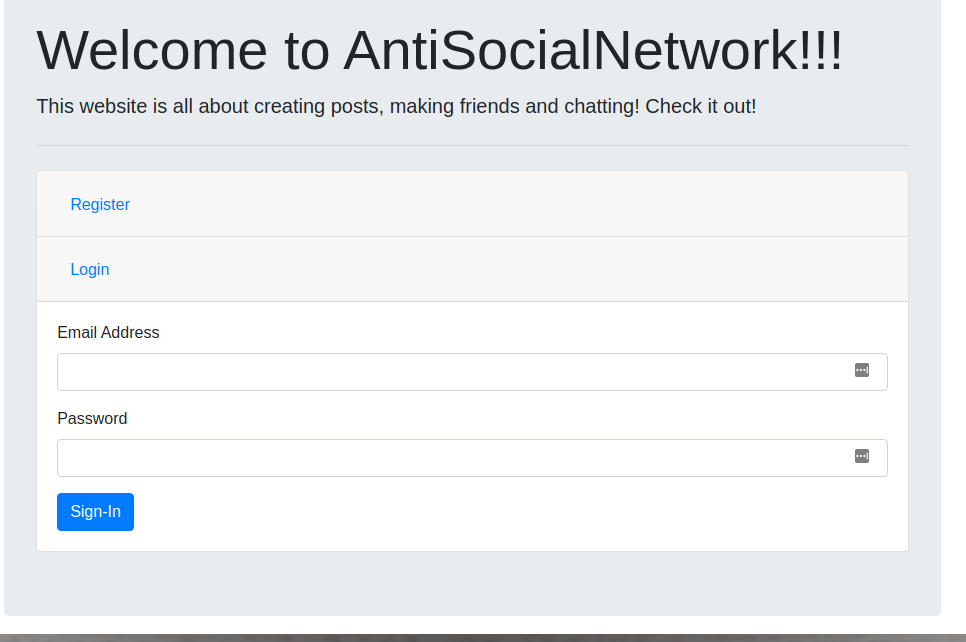
\includegraphics[width=\linewidth]{welcome_page_login.png}
            \end{figure}
        \end{frame}
        
        \begin{frame}[fragile]{Zakładka \textit{Posts}}
            \begin{figure}
                \centering
                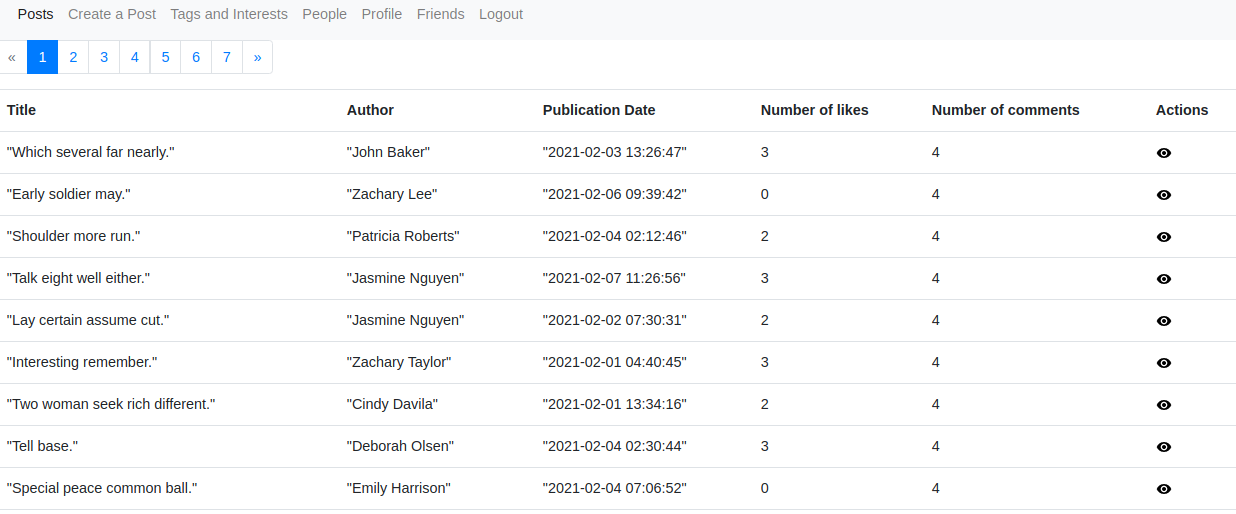
\includegraphics[width=\linewidth]{posts.png}
            \end{figure}
        \end{frame}
        
        \begin{frame}{Przykładowy post - część 1/2}
            \begin{figure}
                \centering
                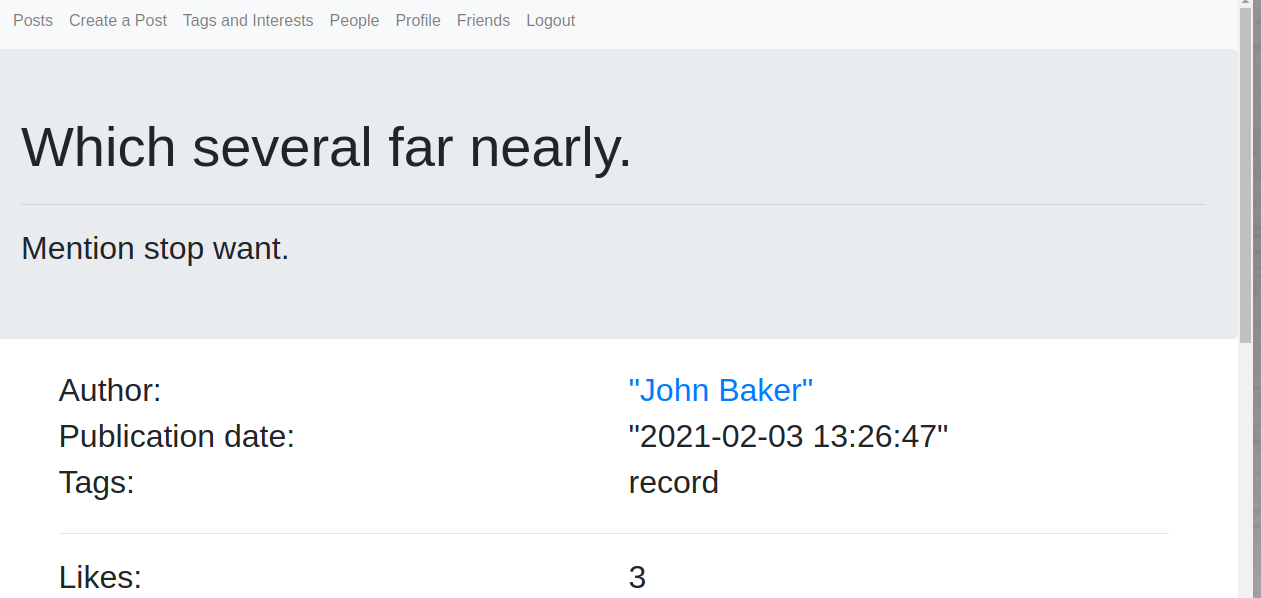
\includegraphics[width=\linewidth]{example_post_part_1.png}
            \end{figure}
        \end{frame}
        
        \begin{frame}{Przykładowy post - część 2/2}
            \begin{figure}
                \centering
                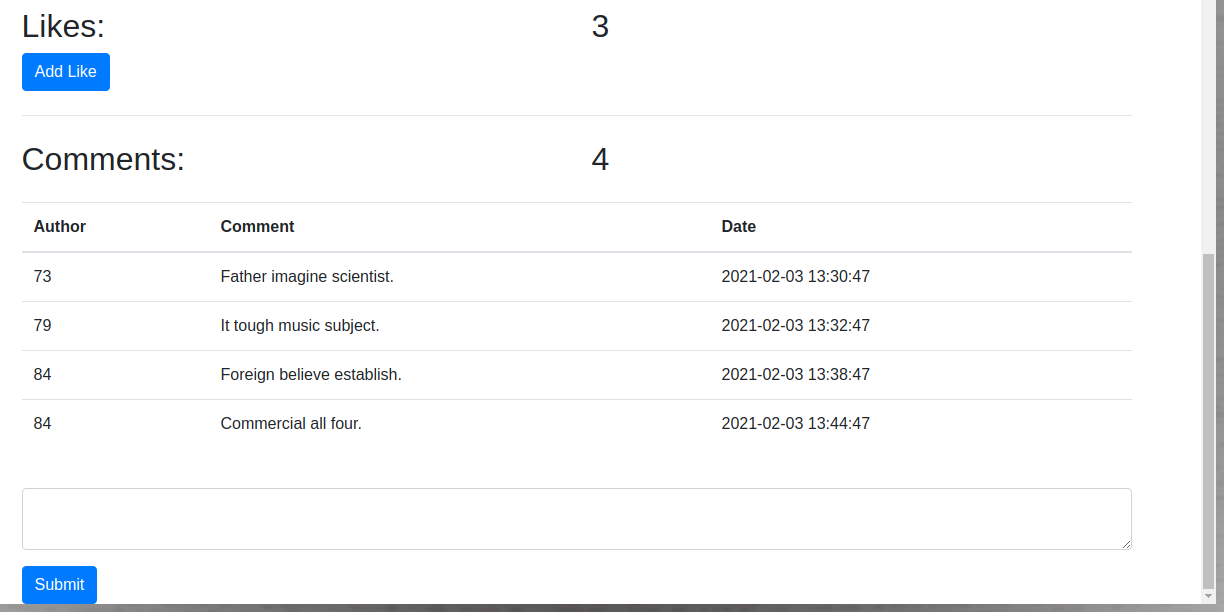
\includegraphics[width=\linewidth]{example_post_part_2.png}
            \end{figure}
        \end{frame}
        
        \begin{frame}{Tworzenie postów}
            \begin{figure}
                \centering
                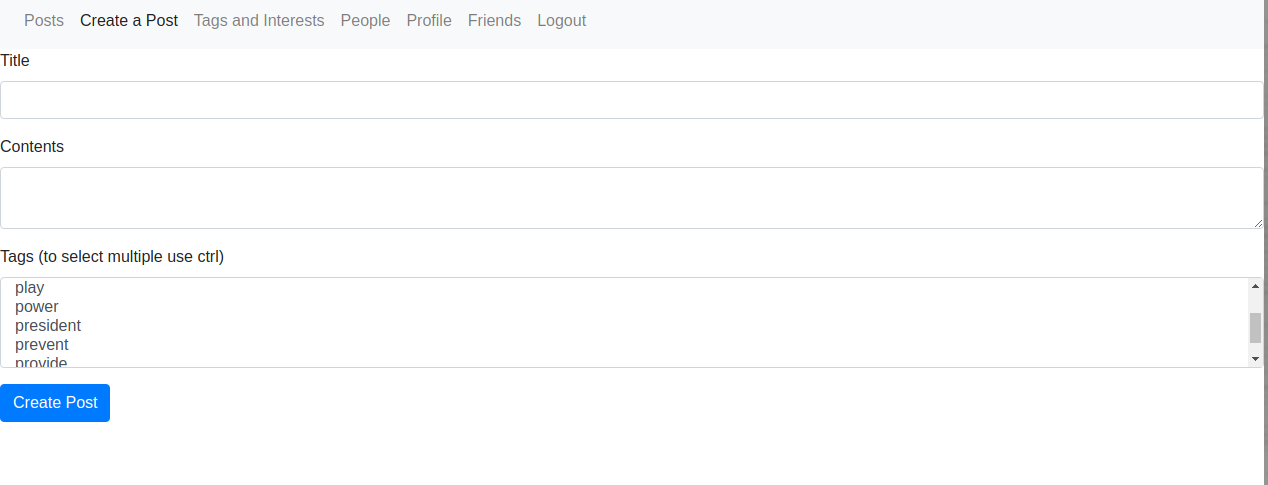
\includegraphics[width=\linewidth]{post_creation.png}
            \end{figure}
        \end{frame}
        
        \begin{frame}{Zakładka \textit{People}}
            \begin{figure}
                \centering
                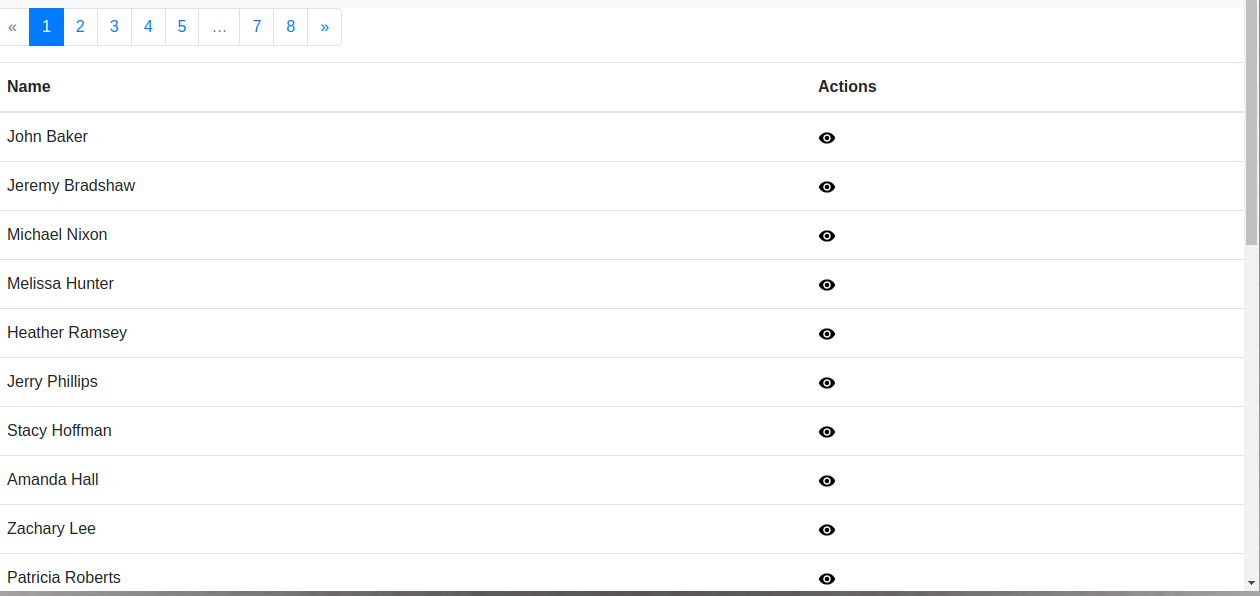
\includegraphics[width=\linewidth]{people.png}
            \end{figure}
        \end{frame}
        
        \begin{frame}{Przykładowy profil}
            \begin{figure}
                \centering
                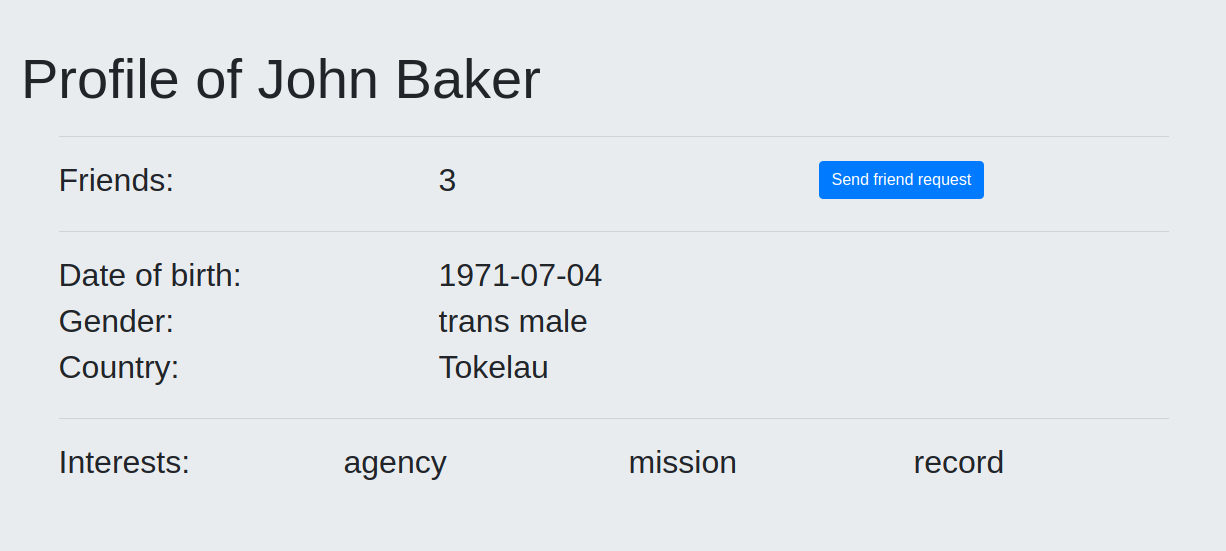
\includegraphics[width=\linewidth]{example_profile.png}
            \end{figure}
        \end{frame}
        
        \begin{frame}{Zakładka \textit{Friends}}
            \begin{figure}
                \centering
                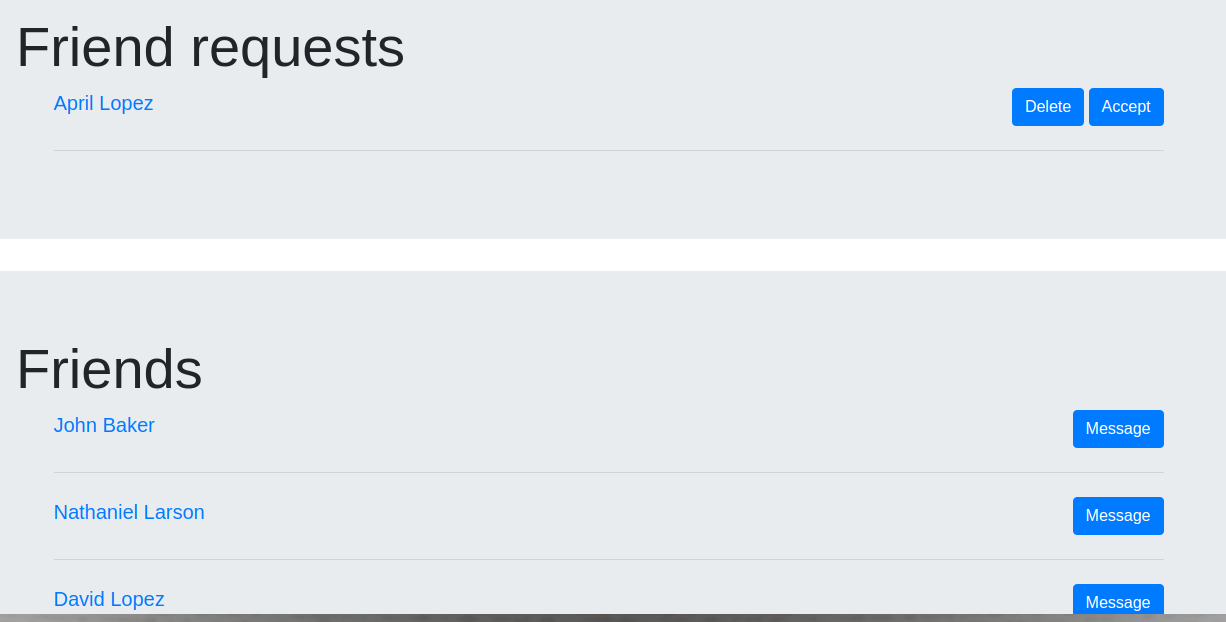
\includegraphics[width=\linewidth]{friends.png}
            \end{figure}
        \end{frame}
        
        \begin{frame}{Przykładowe wiadomości}
            \begin{figure}
                \centering
                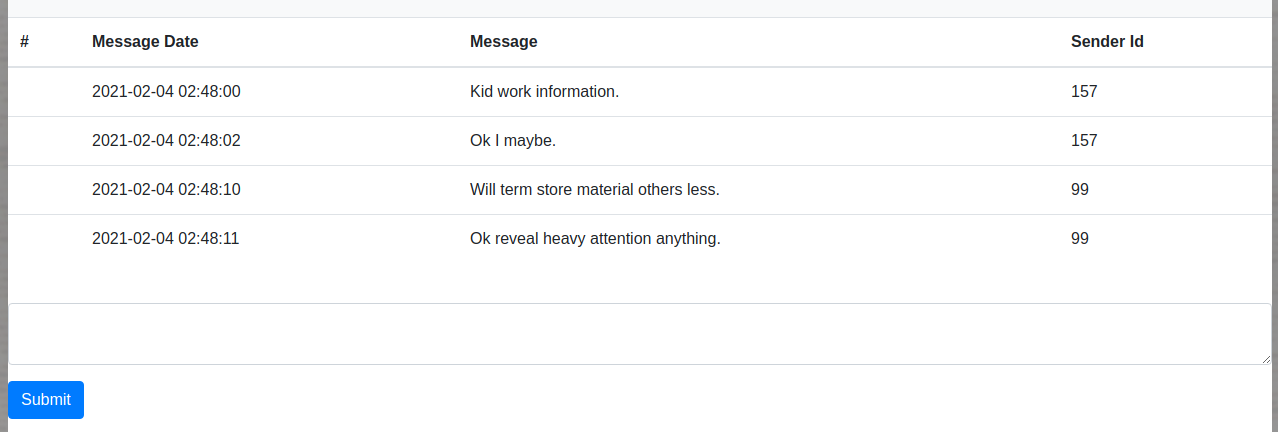
\includegraphics[width=\linewidth]{messages.png}
            \end{figure}
        \end{frame}
        
        \begin{frame}{Zakładka \textit{Tags and Interests} -- część 1/2}
            \begin{figure}
                \centering
                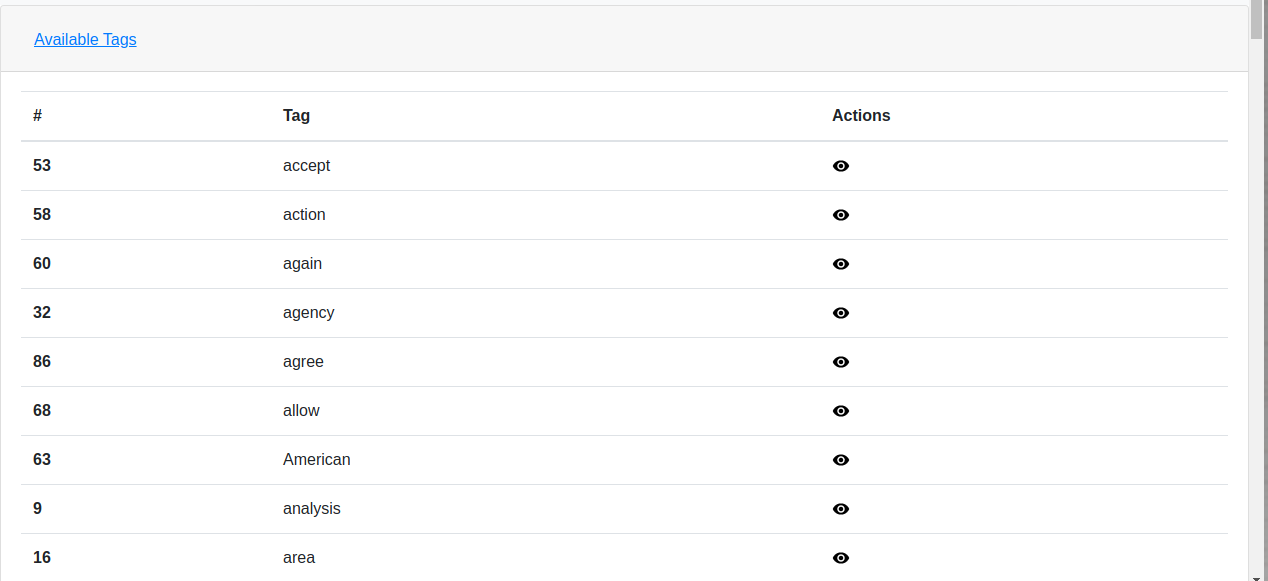
\includegraphics[width=\linewidth]{available_tags.png}
            \end{figure}
        \end{frame}
        
        \begin{frame}{Zakładka \textit{Tags and Interests} -- część 2/2}
            \begin{figure}
                \centering
                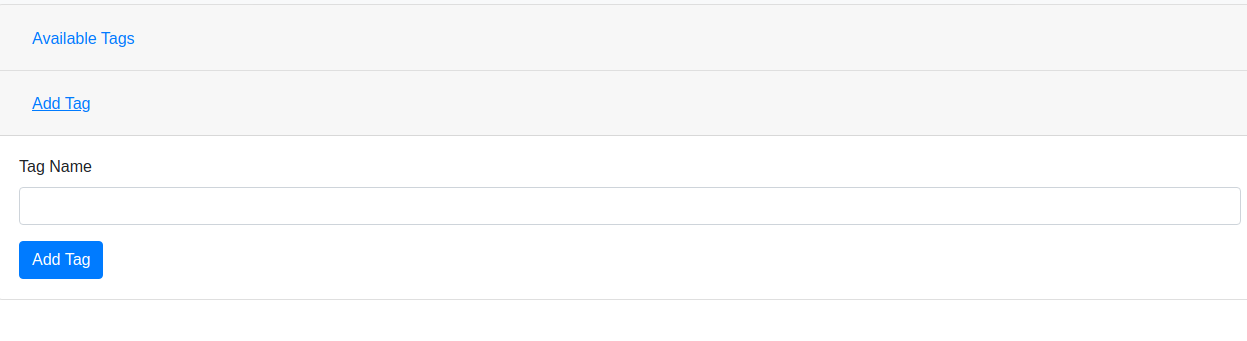
\includegraphics[width=\linewidth]{tag_creation.png}
            \end{figure}
        \end{frame}
        
        \begin{frame}{Używanie tagów}
            \begin{figure}
                \centering
                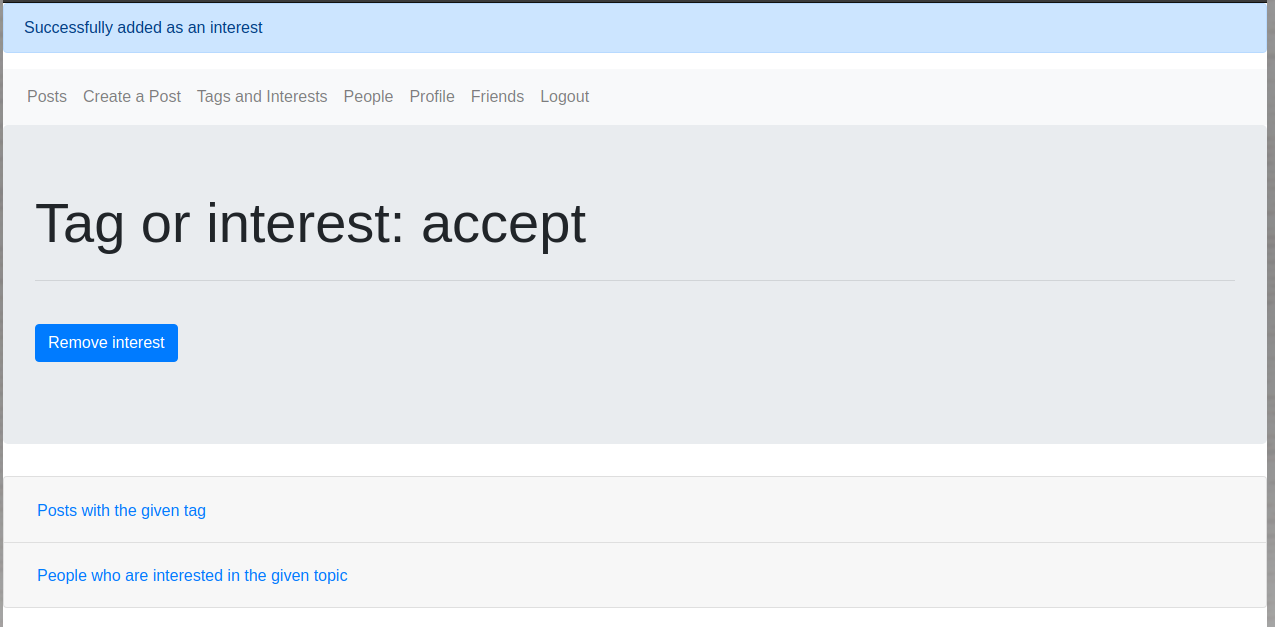
\includegraphics[width=\linewidth]{interests.png}
            \end{figure}
        \end{frame}
    \section{Szczegóły techniczne}
        \begin{frame}{Użyte języki / biblioteki}
            \begin{itemize}
                \item Tworzenie tabel, bazy danych, kluczy -- PostgreSQL
                \item Generowanie danych, wyzwalacze -- PL/Python
                \begin{itemize}
                    \item Szyfrowanie haseł -- biblioteka \textit{bcrypt}
                    \item Przykładowe dane -- biblioteka \textit{faker}
                \end{itemize}
                \item Interfejs graficzny -- Python
                \begin{itemize}
                    \item Poruszanie się pomiędzy zakładkami -- biblioteka \textit{flask}
                    \item Formularze -- biblioteki \textit{wtforms} i \textit{flask-wtforms}
                    \item Wyświetlanie tabel, przycisków, formularzy -- biblioteka \textit{bootstrap-flask}
                    \item Interakcja z bazą danych -- biblioteka \textit{flask-sqlalchemy}
                \end{itemize}
                \item Wyświetlanie stron -- Jinja2 (część flaska, połączenie htmla i pythona)
            \end{itemize}
        \end{frame}
        
    \section{Koniec}
        \begin{frame}
            \centering \LARGE
            \emph{Dziękuję za Uwagę!}
        \end{frame}
\end{document}
